\documentclass{ITESO-Reporte}
\usepackage[spanish]{babel}
\usepackage[sfdefault]{carlito}
\usepackage{csquotes}
\usepackage[style=apa, backend=biber]{biblatex}
    \DefineBibliographyStrings{spanish}{% Cambiado "et al." a italicas
    andothers = {\em et\addabbrvspace al\adddot}
    }
\usepackage{lipsum}

\addbibresource{biblio.bib}
\addto\captionsspanish{\renewcommand*{\contentsname}{\color{azuliteso1}\large\bfseries Tabla de contenidos}} % Cambiar el título de \tableofcontents

\newcommand{\toprow}[1]{\multicolumn{1}{c}{\textbf{#1}}}

\title{Concentración y purificación de pigmentos de espinaca (\textit{Spinacia oleracea}) con columna cromatográfica}

\author[a]{Roberto Olvera-Hernández} % Autor principal siempre va a al inicio.
\author[a]{Brenda F.L. Macias-Viera}
\author[a]{Juan P. Martínez-Montaño}
\author[a]{Carlos A. Vázquez-Meza}
\date{} % Se recomienda dejar vacío para no imprimir la fecha en la zona de título.

\mainemail{ib721045@iteso.mx} % E-mail de autor(a) principal.
\mylab{Bioseparaciones}{PTI2329N} % Nombre del laboratorio

\affil[a]{Ingeniería en biotecnología, \itesoinfo}

\begin{document}

\maketitle % Imprimir título.
    \nocite{*} % Solo para imprimir bibliografía sin escribir (\parencite{}).
    {\small \tableofcontents} % Crear tabla de contenidos con letra más pequeña (\small).
    \thispagestyle{firstpage} % Definir encabezado de la primera página.

%%% Inicio del documento
\begin{abstract}\label{abstract}
    Mediante la técnica de cromatografía se logró separar los diversos componentes de los pigmentos de espinaca con el uso de distintas fases móviles de solventes orgánicos que permitieron obtener beta-carotenos, así como clorofilas a y b. Las propiedades moleculares de los pigmentos en la muestra fueron separados y concentrados dependiendo de su afinidad en la fase móvil, no obstante, no se lograron obtener la totalidad de los pigmentos.
\end{abstract} 
\newpage

\section{Introducción}\label{intro}

La cromatografía es una técnica física que se utiliza para la separación de componentes de un compuesto, de manera que, al separarlos, permitan ser reconocidos. Esta se divide en dos fases, la fase estacionaria y la fase móvil. La fase estacionaria, como bien lo dice su nombre, es el compuesto que permanece dentro de la columna de cromatográfica mientras que la fase móvil es la sustancia que se mueve en una dirección y sentido determinado de la fase estacionaria \parencite{Sgariglia2010}. 

La cromatografía de columna permite aislar compuestos de una mezcla. Ese realiza mediante el uso de un tubo cilíndrico vertical, la cual sería nuestra columna de vidrio, donde en su interior lleva un soporte sólido adsorbente actuando de fase estacionaria y por donde pasa la fase móvil.

De forma general la cromatografía por columna es usada para separar proteínas y su separación depende de la matriz con que esté hecha la fase estacionaria permitiendo o no la interacción con la matriz y su retención y posterior aislamiento.

\section{Materiales}\label{materiales}

\begin{table}[H]
    \centering
    \caption{Reactivos utilizados en la práctica.}
    %\resizebox{\columnwidth}{!}{
    \begin{tabular}{lrc}
        \toprule

        \multicolumn{1}{c}{\textbf{Reactivo}} & \multicolumn{1}{c}{\textbf{Cantidad}} & \multicolumn{1}{c}{\textbf{Unidad}}\\ \hline
        \ch{C2H6O_{(EtOH)}}  & \num{14} & \si{\ml} \\
        \ch{C4H8O2_{(AcEt)}} & \num{20} & \si{\ml} \\
        \ch{C6H14_{(Hex)}}   & \num{41} & \si{\ml} \\
        \ch{CH2Cl2}        & \num{20} & \si{\ml} \\
        \ch{dH2O}          & \num{20} & \si{\ml} \\
        Hoja de espinaca   &  \num{1} & \si{g}   \\
        \ch{Na2SO4}        &  \num{1} & \si{g}   \\
        Sílica gel (60)    &  \num{2} & \si{g}   \\

        \bottomrule
    \end{tabular}
    %}
    \label{tab:reactivos}
\end{table} % Reactivos

\begin{table}[H]
    \centering
    \caption{Materiales utilizados en la práctica.}
    \resizebox{\columnwidth}{!}{
    \begin{tabular}{lrc}
        \toprule
        \multicolumn{1}{c}{\textbf{Material}} & \multicolumn{1}{c}{\textbf{Descripción}} & \multicolumn{1}{c}{\textbf{Cantidad}}\\ \hline
            Agitador de   vidrio     & -                            & \num{1}   \\
            Algodón                  & -                            & \num{1}   \\
            Asa   bacteriológica     & -                            & \num{1}   \\
            Campana de extracción    & -                            & -   \\
            Espátula   acanalada     & -                            & \num{1}   \\
            Filtro                   & -                            & \num{1}   \\
            Gradilla                 & Tubos de ensayo              & \num{1}   \\
            Manguera MasterFlex   14 & D. interno (\qty{16}{\mm})   & \qty{5}{\cm} \\
            Matraz   Erlenmeyer      & \qty{250}{\ml}               & \num{1}   \\
            Micropipeta              & \qty{10}{\micro\l}           & \num{1}   \\
            Micropipeta              & \qty{100}{\micro\l}          & \num{1}   \\
            Micropipeta              & \qty{1000}{\micro\l}         & \num{1}   \\
            Microplaca               & 96 pocillos                  & \num{1}   \\
            Papel aluminio           & -                            & \num{1}   \\
            Pera de   decantación    & \qty{250}{\ml}               & \num{1}   \\
            Pinza de 3   dedos       & -                            & \num{1}   \\
            Pipeta                   & \qty{1}{\ml}                 & \num{1}   \\
            Pipeta                   & \qty{5}{\ml}                 & \num{2}   \\
            Pipeta                   & \qty{10}{\ml}                & \num{2}   \\
            Pipeta Pasteur           & de vidrio                    & \num{2}   \\
            Probeta                  & \qty{100}{\ml}               & \num{1}   \\
            Probeta                  & \qty{10}{\ml}                & \num{1}   \\
            Rack de puntas           & \qty{10}{\micro\l}           & \num{1}   \\
            Rack de puntas           & \qty{100}{\micro\l}          & \num{1}   \\
            Rack de puntas           & \qty{1000}{\micro\l}         & \num{1}   \\
            Soporte universal        & -                            & \num{1}   \\
            Tijeras                  & -                            & \num{1}   \\
            Tubo de ensayo           & \qty{5}{\ml}                 & \num{5}   \\
            Tubo de ensayo           & \qty{10}{\ml}                & \num{7}   \\
            Vaso de   precipitado    & \qty{50}{\ml}                & \num{1}   \\
        \bottomrule
    \end{tabular}
    }
    \label{tab:materiales}
\end{table} % Materiales

\newpage
\section{Métodos} \label{metodos}
\subsection{Preparación del extracto} \label{extract}

Hojas de espinaca (\textit{Spinacia oleracea}) fueron compradas en supermercado. Se retiraron tallo y venas para pesar \qty{1}{\g} de hoja partida en trozos de aproximadamente \qty{0.5}{\square\cm}. Los trozos de hoja fueron macerados junto con \qty{3}{\ml} de metanol para romper la pared celular y liberar los pigmentos (figura \ref{fig:extract}), para posteriormente agregar bajo campana \qty{6}{\ml} de hexano dividido en 2 alícuotas para realizar la extracción de los pigmentos.

\begin{figure}[htpb]
    \centering
    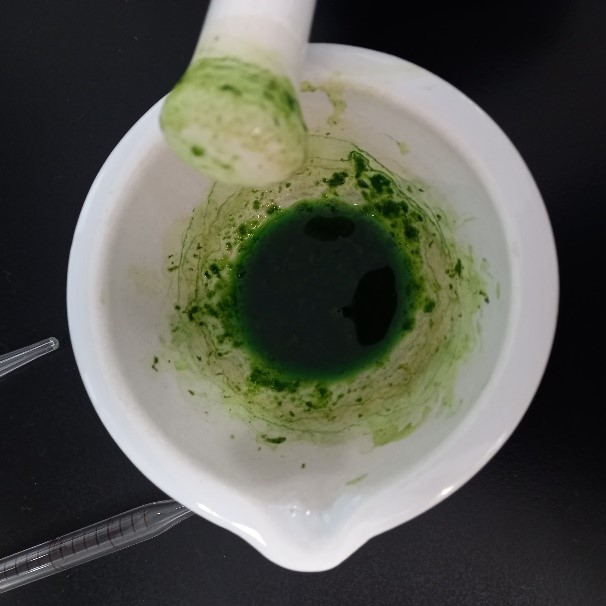
\includegraphics[width=0.9\columnwidth]{figuras/extract.jpg}
    \caption{Extracto de macerado de espinaca con hexano.}
    \label{fig:extract}
\end{figure}

Con la ayuda de un papel filtro, el extracto fue transferido a una pera de decantación; hubo pérdidas por capilaridad en el papel filtro. Al resto de la muestra se le volvieron a adicionar \qty{6}{\ml} de hexano para recuperar los pigmentos restantes.

Dentro de la pera se agregaron \qty{10}{\ml} de agua destilada para lavar el extracto que quedó adherido en las paredes, meciendo lentamente la pera. Después de que se formaran las fases, el agua fue recuperada en un matraz para ser desechada, y se repitió el lavado. El extracto fue recuperado en un matraz de \qty{50}{\ml} y secado con \qty{1}{\g} de \ch{Na2SO4}. Finalmente, se concentró el extracto por evaporación con una manguera de vacío, resultando en una extracción de aproximadamente \qty{1.5}{\ml} (figura \ref{fig:final-extract}).

\begin{figure}[htpb]
    \centering
    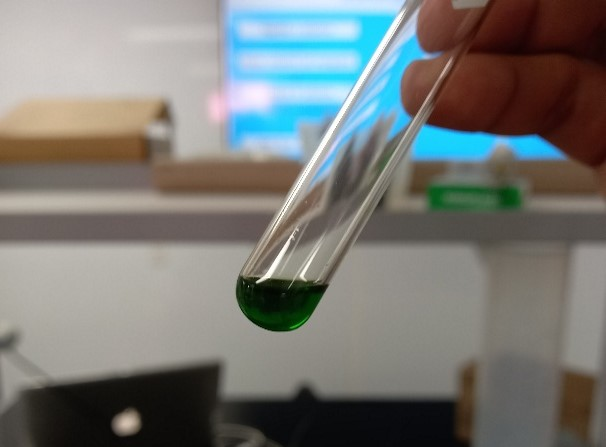
\includegraphics[width=0.9\columnwidth]{figuras/final_extract.jpg}
    \caption{Extracción final y concentrada de pigmentos con hexano.}
    \label{fig:final-extract}
\end{figure}

\subsection{Preparación de las fases móviles}\label{fases moviles}

Se prepararon \qty{10}{\ml} de cada fase móvil bajo campana en tubos de ensayo de \qty{20}{\ml} que fueron etiquetados.

\begin{enumerate}
    \setlength{\itemsep}{0pt}
    \item \ch{C6H14}
    \item \ch{C6H14}:\ch{CH2Cl2} (9:1)
    \item \ch{CH2Cl2}
    \item \ch{CH2Cl2}:\ch{C4H8O2} (9:1)
    \item \ch{C4H8O2}
    \item \ch{C4H8O2}:\ch{C2H6O} (9:1)
    \item \ch{C2H6O}
\end{enumerate}

\subsection{Cromatografía de columna}\label{cromatografia}

Se realizo la elección y preparación de la fase móvil y fase estacionaria en donde se colocó un algodón para posteriormente colocarle la sílica gel, para formar la mezcla del absorbente con el eluyente para formar la fase estacionaria, la cual quedo compactada dentro de la columna. Para la aplicación de la muestra se colocó la extracción realizada de los pigmentos de espinaca 0.5 mL para disolverla y hacerla pasar a través de la columna con la ayuda de una pipeta, en la corrida de la cromatografía y elución de los componentes se colocó la muestra y la fase estacionaria, para correr la fase móvil (disolvente) a través de la columna esto ayudo a lavar los distintos componentes (eluatos) de la muestra según su afinidad por alguna de las fases (elución) móviles colocadas.

Para la detección de los componentes los analitos recogidos fueron recolectados en un tubo de manera manual por fracciones para poder almacenar los compuestos separados pues hubo distintas fracciones que fueron recuperadas atravesando la cromatografía de capa delgada para su posterior análisis.

\section{Resultados}\label{resultados}

\begin{figure}[htpb]
    \centering
    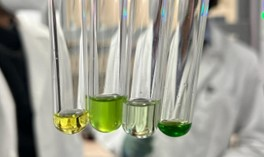
\includegraphics[width=0.9\columnwidth]{figuras/pigments.jpg}
    \caption{Pigmentos recuperados por columna cromatográfica. En orden de izquierda a derecha: beta-caroteno, clorofila a, clorofila b, extracto.}
    \label{fig:pigments}
\end{figure}

\begin{table}[htpb]
    \centering
    \caption{Identificación de pigmentos.}
    \resizebox{\columnwidth}{!}{
    \begin{tabular}{lcc}
        \toprule
        \toprow{Pigmento} & \toprow{Color} & \toprow{Absorbancia (nm)}\\ \hline
        Clorofila a & Verde & 630\\
        Clorofila b & Azul-verde & 650\\
        Xantofilas & Amarillo & 450\\
        beta-caroteno & Naranja-amarillo & 448 \\
        \bottomrule
    \end{tabular}
    }
    \label{tab:pigment}
\end{table}

Para poder separar los distintos pigmentos recuperados, fue necesario probar las diversas fases móviles preparadas para poder observar cual era más afín a los componentes encontrados, realizando una cromatografía de capa fina. Como se puede observar en la figura 3, la cantidad de clorofila recuperada fue en mayor proporción ya que la clorofila constituye la mayor parte de color verde en las plantas, las xantofilas, las cuáles son de color amarillo estas se obtuvieron en pequeña cantidad y hubo un pigmento que no se logró recuperar ya que no fue visible a simple vista.

\section{Discusión de resultados}

{\color{darkgray}\bfseries Brenda F.L Macías-Vera:}\hspace{1em}
La técnica de cromatografía es una de las más utilizadas para separar componentes en la industria para determinar los distintos componentes de una sustancia, como fue aplicado en la práctica se recuperaron distintos componentes de los pigmentos de espinaca, estos son caracterizados por absorber luz (clorofila, carotenoides). Las distintas polaridades permitieron que las fases móviles a distintas concentraciones se recuperaran implementando con hexano, cloruro de metilo, acetato de etilo y metanol por la misma afinidad que presentaron se separaron logrando recuperar las fracciones de Xantofilas, Clorofila b y a.

{\color{darkgray}\bfseries Juan P. Martínez-Montaño:}\hspace{1em}
La interacción de los pigmentos con relación a su afinidad por la fase móvil permitió la separación de diversos tipos de pigmentos contenidos en la hoja de espinaca, donde pudimos obtener una mayor concentración de pigmentos de clorofila “a”, seguidos de la clorofila “b” y por último, contenido de beta-carotenos, no obstante, se perdió en el proceso uno de los pigmentos “leaf-stain” al no ser del todo visibles al momento de procesar la fase móvil con acetato de etilo.

{\color{darkgray}\bfseries Roberto Olvera-Hernández:}\hspace{1em}
Usando un gradiente de polaridad, se lograron purificar 3 pigmentos: carotenos, clorofila a y b. El orden de migración de los metabolitos y sus respectivas fases móviles coinciden con lo reportado por \textcite{Khalyfa1992}. El uso de hexano como solvente para la migración de carotenoides tuvo buenos resultados como mencionaron \textcite{Mussagy2018} en su revisión.

{\color{darkgray}\bfseries Carlos A. Vázquez-Meza:}\hspace{1em}
La cromatografía es un método físico de separación en el que se utilizan dos fases (fija y móvil) y la afinidad de una especie química para asociarse más con una que con otra. El objetivo es separar pequeñas cantidades de una mezcla. Este método es especialmente adecuado para las mezclas coloreadas. En el segundo grado, la fase móvil es líquida y la fase fija es sólida.

Como cada componente es fácilmente absorbido por la fase fija y disuelto en la fase móvil, su migración a través de la columna será a una determinada velocidad. A veces es necesario utilizar varios disolventes, uno tras otro, para arrastrar lo mejor posible los distintos componentes.


\section{Conclusiones}

{\color{darkgray}\bfseries Brenda F.L Macías-Vera:}\hspace{1em}
La cromatografía es una técnica de separación y análisis para separar diversos compuestos presentes en una muestra utilizando una fase estacionaria eluida con la fase móvil por lo que puede ser aplicado para separar pigmentos u otras soluciones que tengan afinidad a la fase móvil por lo que es importante caracterizar y saber cuáles son las que tienen alta polaridad en este caso se utilizó la silica gel puesto que posee esta característica y además es porosa por lo que permite que la acción capilar de la fase móvil se sienta atraída para que al interactuar con la muestra siendo atraída o no. La determinación para la composición de las hojas de espinaca posee interacción dipolo-dipolo lo cual les da una mayor polaridad.

{\color{darkgray}\bfseries Juan P. Martínez-Montaño:}\hspace{1em}
En los procesos de separación podemos identificar variables que nos permitan tomar decisiones más asertivas para seleccionar y manejar correctamente las técnicas de concentración y purificación. Entre estas, podemos encontrar la afinidad de las partículas de interés en nuestra alícuota, así como el tamaño per se del compuesto de interés, y de esta manera, lograr mayores porcentajes de recuperación. 

{\color{darkgray}\bfseries Roberto Olvera-Hernández:}\hspace{1em}
El manejo de este equipo de escala laboratorio y usar componentes coloridos/visuales ayudó a comprender mejor los fundamentos de la cromatografía por columna. Resultó ser un método de separación sencillo y de alta eficiencia. Una mejor forma de filtrado o técnica para evitar pérdidas por capilaridad en el papel filtro debería ser tomada en cuenta.

{\color{darkgray}\bfseries Carlos A. Vázquez-Meza:}\hspace{1em}
La Cromatografía en columna es un método muy útil para la separación de porciones considerables de compuestos de alguna mezcla que tengamos. Es de suma importancia tomar en cuenta todas las precauciones para asegurar el triunfo de este procedimiento pues es bastante largo y cualquier error podría alterar los resultados obtenidos.


\section{Perspectivas}\label{perspectivas}

En la industria, existen numerosas aplicaciones en la extracción de pigmentos ya qué en la mayoría de los casos, estos presentan moléculas de interés que pueden ser purificadas y concentradas para su comercialización, como lo son los carotenoides, que son ricos en vitamina B, o en algunos compuestos ricos en antioxidantes, los cuales generan un gran valor nutricional y a su vez, monetario.

Existen diversos métodos para la extracción de pigmentos o moléculas de interés, pero es importante conocer la naturaleza de los metabolitos que se desean concentrar, ya que dependen de la afinidad que tengan a las distintas fases móviles que podamos emplear o incluso, la variación de métodos que nos permitan obtener mejores resultados en el factor de recuperación.


\section{Contribución de los autores}
{\color{darkgray}\bfseries Brenda F.L Macías-Vera:}\hspace{1em}
Realizó la contribución para la preparación del extracto de espinaca, Escribió \textit{\ref{cromatografia} Cromatografía de columna} y \textit{\ref{resultados} Resultados}.

{\color{darkgray}\bfseries Juan P. Martínez-Montaño:}\hspace{1em}
Realizó la formulación de las fases móviles y apoyó en la operación de la columna. Escribió \textit{\ref{perspectivas} Perspectivas} y \textit{Resumen}.

{\color{darkgray}\bfseries Roberto Olvera-Hernández:}\hspace{1em}
Operó columna cromatográfica. Preparó el extracto de espinaca. Escribió \textit{\ref{materiales} Materiales} y \textit{\ref{metodos} Métodos}.

{\color{darkgray}\bfseries Carlos A. Vázquez-Meza:}\hspace{1em}
Escribió \textit{\ref{intro} Introducción}.

\printbibliography[title=Referencias citadas]

\end{document}